\documentclass[a4paper,11pt]{article}
\usepackage{hyperref} % Added for hyperlinks
\hypersetup{
    colorlinks=true, % Set to true to remove box
    linkcolor=blue,
    filecolor=magenta,      
    urlcolor=blue,
}
\usepackage{latexsym}
\usepackage{xcolor}
\usepackage{float}
\usepackage{ragged2e}
\usepackage[empty]{fullpage}
\usepackage{wrapfig}
\usepackage{lipsum}
\usepackage{tabularx}
\usepackage{titlesec}
\usepackage{geometry}
\usepackage{marvosym}
\usepackage{verbatim}
\usepackage{enumitem}
\usepackage{fancyhdr}
\usepackage{fontawesome5}
\usepackage{multicol}
\usepackage{graphicx}
\usepackage{cfr-lm}
\usepackage[T1]{fontenc}
\setlength{\multicolsep}{0pt} 
\pagestyle{fancy}
\fancyhf{} % clear all header and footer fields
\fancyfoot{}
\renewcommand{\headrulewidth}{0pt}
\renewcommand{\footrulewidth}{0pt}
\geometry{left=1.4cm, top=0.8cm, right=1.2cm, bottom=1cm}

\usepackage[most]{tcolorbox}
\tcbset{
    frame code={},
    center title,
    left=0pt,
    right=0pt,
    top=0pt,
    bottom=0pt,
    colback=gray!20,
    colframe=white,
    width=\dimexpr\textwidth\relax,
    enlarge left by=-2mm,
    boxsep=4pt,
    arc=0pt,outer arc=0pt,
}

\urlstyle{same}

\raggedright
\setlength{\tabcolsep}{0in}

% Sections formatting
\titleformat{\section}{
  \vspace{-4pt}\scshape\raggedright\large
}{}{0em}{}[\color{black}\titlerule \vspace{-7pt}]

% Custom commands
\newcommand{\resumeItem}[2]{\item{\textbf{#1}{\hspace{0.5mm}#2 \vspace{-0.5mm}}}}

\newcommand{\resumePOR}[3]{\vspace{0.5mm}\item
    \begin{tabular*}{0.97\textwidth}[t]{l@{\extracolsep{\fill}}r}
        \textbf{#1}\hspace{0.3mm}#2 & \textit{\small{#3}} 
    \end{tabular*}
    \vspace{-2mm}
}

\newcommand{\resumeSubheading}[4]{\vspace{0.5mm}\item
    \begin{tabular*}{0.98\textwidth}[t]{l@{\extracolsep{\fill}}r}
        \textbf{#1} & \textit{\footnotesize{#4}} \\
        \textit{\footnotesize{#3}} &  \footnotesize{#2}\\
    \end{tabular*}
    \vspace{-2.4mm}
}

\newcommand{\resumeProject}[4]{\vspace{0.5mm}\item
    \begin{tabularx}{0.98\textwidth}[t]{l@{\extracolsep{\fill}}r}
        \textbf{#1} & \textit{\footnotesize{#3}} \\
        \multicolumn{2}{@{}p{\dimexpr\linewidth-2\tabcolsep}@{}}{\small{\textit{#2}}} \\
        \multicolumn{2}{@{}p{\dimexpr\linewidth-2\tabcolsep}@{}}{\small{#4}}
    \end{tabularx}
    \vspace{-2.4mm}
}

\newcommand{\resumeSubItem}[2]{\resumeItem{#1}{#2}\vspace{-4pt}}

\renewcommand{\labelitemi}{$\vcenter{\hbox{\tiny$\bullet$}}$}

\newcommand{\resumeSubHeadingListStart}{\begin{itemize}[leftmargin=*,labelsep=0mm]}
\newcommand{\resumeHeadingSkillStart}{\begin{itemize}[leftmargin=*,itemsep=1.7mm, rightmargin=2ex]}
\newcommand{\resumeItemListStart}{\begin{justify}\begin{itemize}[leftmargin=3ex, rightmargin=2ex, noitemsep,labelsep=1.2mm,itemsep=0mm]\small}

\newcommand{\resumeSubHeadingListEnd}{\end{itemize}\vspace{2mm}}
\newcommand{\resumeHeadingSkillEnd}{\end{itemize}\vspace{-2mm}}
\newcommand{\resumeItemListEnd}{\end{itemize}\end{justify}\vspace{-2mm}}
\newcommand{\cvsection}[1]{%
\vspace{2mm}
\begin{tcolorbox}
    \textbf{\large #1}
\end{tcolorbox}
    \vspace{-4mm}
}

\newcolumntype{L}{>{\raggedright\arraybackslash}X}%
\newcolumntype{R}{>{\raggedleft\arraybackslash}X}%
\newcolumntype{C}{>{\centering\arraybackslash}X}%

\newcommand{\name}{Subhranil Karmakar} % Your Name
\newcommand{\course}{B. Tech} % Your Program
\newcommand{\roll}{2028035} % Your Roll No.
\newcommand{\phone}{9883279562} % Your Phone Number
\newcommand{\emaila}{subhranilkarmakar00@gmail.com} %Email 1
\newcommand{\emailb}{2028035@kiit.ac.in} %Email 2

\begin{document}
\parbox{2.35cm}{%
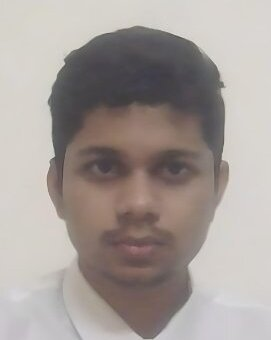
\includegraphics[width=2cm,clip]{Passport Photo_Subhranil Karmakar c.jpeg}
}
\parbox{\dimexpr\linewidth-2.8cm\relax}{
\begin{tabularx}{\linewidth}{L r} \\
  \textbf{\Large \name} & {\raisebox{0.0\height}{\footnotesize \faPhone}\ +91-\phone}\\
  {Roll No.: \roll} & \href{mailto:\emaila}{\raisebox{0.0\height}{\footnotesize \faEnvelope}\ {\emaila}} \\
  \course &  \href{mailto:\emailb}{\raisebox{0.0\height}{\footnotesize \faEnvelope}\ {\emailb}}\\
  {Computer Science and System Engineering} &  \href{https://github.com/Subhranil2152}{\raisebox{0.0\height}{\footnotesize \faGithub}\ {GitHub Profile}} \\
  {Kalinga Institute of Industrial Technology, Bhubaneshwar} & \href{https://www.linkedin.com/in/subhranil-karmakar-526311200/}{\raisebox{0.0\height}{\footnotesize \faLinkedin}\ {LinkedIn Profile}}\\
  
\end{tabularx}
}

\section{\textbf{Education}}
\resumeSubHeadingListStart
    \resumeSubheading
      { Kalinga Institute of Industrial Technology, Bhubaneshwar}{CGPA/Percentage: 8.97}
      {B.Tech in Computer Science and System Engineering}{2020-2024}
    \resumeSubheading
      { Apeejay School Saltlake, Kolkata}{CGPA/Percentage: 90}
      {CBSE, West Bengal}{2020}
    \resumeSubheading
      { Saint Francis Xavier School, Kolkata}{CGPA/Percentage: 90}
      {ICSE, West Bengal}{2018}
\resumeSubHeadingListEnd
\vspace{-7mm}
\section{\textbf{Experience}}
\resumeSubHeadingListStart
    \resumeSubheading
      { HighRadius  Technologies}{Bhubaneshwar}
      {Summer Intern \href{https://drive.google.com/file/d/1danat5Qjfukbp-m4nCk54QaBW7c6rWsj/view?usp=drive_link}{\textcolor{blue}{Drive}}}{22nd May to 23rd June } % Added hyperlink
      \vspace{-2.0mm}
      \resumeItemListStart
        \item {Conducted machine learning predictions on customer order amounts utilizing regression techniques.}
        \item {Developed and implemented a front-end application using React and Java, resulting in the successful creation of an AI-Enabled FinTech B2B Invoice Management Application.}
      \resumeItemListEnd
    \resumeSubheading
      { HighRadius  Technologies}{Bhubaneshwar}
      {Paid Intern \href{https://drive.google.com/file/d/1nJIgtRqklHgm3Q6YoKwWWvMdyZckGKsL/view?usp=drive_link}{\textcolor{blue}{Drive}}}{12th July May to 24th November } % Added hyperlink
      \vspace{-2.0mm}
      \resumeItemListStart
        \item {Acquired foundational knowledge of the operational dynamics of a Java-based Fintech company.}
        \item {Demonstrated proficiency in working with technologies such as Spring, Struts, Hibernate, Docker, and Kubernetes.}
        \item {Received and successfully executed assignments encompassing ECI Validation, Web Agent Walkthrough, and Scraping.}
      \resumeItemListEnd
\resumeSubHeadingListEnd

\vspace{-8.5mm}

\section{\textbf{Personal Projects}}
\resumeSubHeadingListStart
    \resumeProject
        {\textbf{Full Stack Grocery Store Management WebApp} \href{https://github.com/Subhranil2152/Full-Stack-Grocery-Management-Application}{\textcolor{blue}{GitHub}}} % Added hyperlink
        {A grocery store management application with a three-tier architecture: front end developed using HTML,CSS,JavaScript,Bootstrap. Back end implemented in Python using Flask, and MySQL for the database with a trained chatbot }
        {} % Location Name
    
    \vspace{-6mm}
    \resumeProject
        {\textbf{Drowsiness Detection in Drivers} \href{https://github.com/Subhranil2152/Driver-Drowsiness-Detection}{\textcolor{blue}{GitHub}}} % Added hyperlink
        {Implemented a project to assess drowsiness by comparing aspect ratio calculations of a driver's mouth, eye, and stitch positions against predefined thresholds. Promptly notifying the driver of detected intoxication or drowsiness }
        {} % Location Name
    


    \vspace{-6mm}
    \resumeProject
        {\textbf{Uber Ride Analysis} \href{https://github.com/Subhranil2152/UberDataAnalysis}{\textcolor{blue}{GitHub}}} % Added hyperlink
        {Analyzed customer ride paths for booking patterns, destinations, arrival times, and ride purposes, assessing roundtrip booking feasibility based on patterns }
        {} % Location Name

 

    \vspace{-6mm}
    \resumeProject
        {\textbf{Portfolio Website} \href{https://github.com/Subhranil2152/Portfolio-website}{\textcolor{blue}{GitHub}}} % Added hyperlink
        {Developed a responsive portfolio website for optimal employment presentation, featuring user-friendly feedback and contact forms }
        {} % Location Name

\resumeSubHeadingListEnd

 \vspace{-9mm}
\section{\textbf{Technical Skills and Interests}}
\begin{itemize}[leftmargin=0.05in, label={}, itemsep=0mm]
    \small{
        \item[] \textbf{Community Coding}: 200+ Problems on LeetCode, 3 Star in CodeChef \href{https://leetcode.com/subhranil_2152/}{\textcolor{blue}{LeetCode}} \href{https://www.codechef.com/users/subhranil2152}{\textcolor{blue}{CodeChef}}   
        \item[] \textbf{Languages}: Java, C++, C, HTML, CSS, JavaScript, Python
        \item[] \textbf{Skills}: DSA, OOP, DBMS
        \item[] \textbf{Developer Tools}: GitHub, VS Code, Jupyter Notebook, Linux, Bootstrap
        \item[] \textbf{Certifications}: Amazon Web Services (AWS): AICTE NEAT, AWS Academy Graduate \href{https://drive.google.com/file/d/1gBr-gpUL7rCLDwc39vP0q3KjmySKBiMP/view?usp=sharing}{\textcolor{blue}{Drive}} % Added hyperlinks
        \item[] \textbf{Cloud/Databases}: AWS, MySQL
        \item[] \textbf{Soft Skills}: Time Management, Leadership, Problem-solving, Work Ethic, Creativity, Teamwork
    }
\end{itemize}


\section{\textbf{Conference Papers}}
\begin{itemize}[leftmargin=0.05in, label={}]
    \small{\item{
        \textAn IOT Solution for Cattle Healthcare Monitoring and Tracking \href{https://ieeexplore.ieee.org/document/10053837}{\textcolor{blue}{IEEE}} \href{https://drive.google.com/file/d/15noMKYeeE6e6Ujh-8jzR2arvV1OHwCUP/view?usp=drive_link}{\textcolor{blue}{Drive}} \\ % Added hyperlink
        \textDrowsiness Detection In Drivers \href{https://ieeexplore.ieee.org/document/10431259}{\textcolor{blue}{IEEE}} \href{https://drive.google.com/file/d/1L-rdg8BdFRRNphkvO3UFX1wTpGS6BvXK/view?usp=sharing}{\textcolor{blue}{Drive}} \\ % Added hyperlink
    }}
\end{itemize}
\vspace{-6.5mm}

\end{document}
